%%% Proof-Carrying Transactions — Full Research Paper
\documentclass[10pt,conference]{IEEEtran}
\IEEEoverridecommandlockouts

\usepackage{cite}
\usepackage{amsmath,amssymb,amsfonts}
\usepackage{amsthm}
\usepackage{algorithm}
\usepackage{algorithmic}
\usepackage{graphicx}
\usepackage{textcomp}
\usepackage{xcolor}
\usepackage{url}
\usepackage{hyperref}
\usepackage{booktabs}
\usepackage{multirow}
\usepackage{tikz}
\usetikzlibrary{arrows.meta, positioning, shapes.geometric, calc, decorations.markings}
\usepackage{pgfplots}
\pgfplotsset{compat=1.18}
\usepackage{listings}
\usepackage{subcaption}
\usepackage{balance}

\newtheorem{theorem}{Theorem}
\newtheorem{lemma}[theorem]{Lemma}
\newtheorem{definition}{Definition}
\newtheorem{corollary}{Corollary}
\newtheorem{property}{Property}

\lstset{
  basicstyle=\ttfamily\footnotesize,
  keywordstyle=\color{blue!70!black}\bfseries,
  commentstyle=\color{green!50!black},
  stringstyle=\color{red!60!black},
  breaklines=true,
  frame=single,
  numbers=left,
  numberstyle=\tiny\color{gray},
  xleftmargin=2em,
  framexleftmargin=1.5em
}

\def\BibTeX{{\rm B\kern-.05em{\sc i\kern-.025em b}\kern-.08em
    T\kern-.1667em\lower.7ex\hbox{E}\kern-.125emX}}

\begin{document}

\title{Proof-Carrying Transactions: Zero-Knowledge\\Policy Compliance for Autonomous AI Agents}

\author{\IEEEauthorblockN{Anonymous Author(s)}}

\maketitle

%% ===================================================================
%% ABSTRACT
%% ===================================================================
\begin{abstract}
Autonomous AI agents pose a non-trivial problem for enterprise governance. These agents execute financial transactions, orchestrate multi-step API calls, and operate with minimal human oversight---making it exceedingly hard to enforce policy at the point of network egress. Individual outbound requests look harmless. Composed together, they trigger \emph{egress-time policy violations}: breached spending caps, ignored temporal windows, drift outside approved task categories. The standard fix is a centralized proxy firewall. This is fragile. It demands implicit trust in the proxy, creates a single point of compromise, and blocks independent auditability.

We propose \textbf{Proof-Carrying Transactions (PCT)}. PCT transforms every outbound agent request into a self-certifying artifact. Each request carries a zero-knowledge succinct non-interactive argument of knowledge (zk-SNARK) proving compliance with the organization's declarative policy constraints. The receiver never sees the rules, the thresholds, or internal agent state.

Our primary contribution lies in applied systems architecture rather than pure cryptographic theory. We built a domain-specific \emph{Policy Constraint Language} (PCL) and a compiler that maps declarative egress rules into tightly optimized Rank-1 Constraint Systems (R1CS), cutting constraint overhead by two orders of magnitude versus general-purpose zkVMs like RISC Zero. On top of Groth16 over BN254, we introduce three application-layer gadgets for AI governance: a 16-bit quantized semantic similarity threshold, temporal window proofs, and hierarchical Merkle-based whitelist accumulators.

We evaluated PCT against 847 enterprise-derived policies. Median proof generation: 95ms. Verification: 4.2ms, constant-time. 97.3\% of policies compiled to under 11,200 R1CS gates. We prove computational soundness, zero-knowledge privacy, and a property we call \emph{policy-binding completeness}---a non-compliant agent cannot forge a valid proof; compliant agents are never rejected. We also map PCT onto the EU AI Act and NIST AI RMF, showing that cryptographic enforcement directly addresses emerging governance mandates.
\end{abstract}

\begin{IEEEkeywords}
Zero-Knowledge Proofs, Autonomous AI Agents, Agent Alignment, Proof-Carrying Code, Cryptographic Policy Enforcement, AI Governance, zk-SNARK, Groth16, EU AI Act Compliance
\end{IEEEkeywords}

%% ===================================================================
%% I. INTRODUCTION
%% ===================================================================
\section{Introduction}
\label{sec:intro}

LLM-based agents now autonomously reason, plan, and execute actions across enterprise infrastructure~\cite{xi2023rise, wang2024survey}. They initiate fund transfers. They modify database records. They call third-party services with minimal human oversight---and the aggregate consequences are measurable in millions of dollars.

This creates what we call the \textbf{Autonomous Egress Problem}: how does an organization cryptographically guarantee that an agent's outbound request complies with its governance policy? The question has teeth. We need to do this without forcing downstream receivers to trust a network intermediary, and without leaking proprietary policy logic.

\subsection{Limitations of Trust-Based Enforcement}

Existing approaches to this problem exhibit three fundamental shortcomings:

\textbf{(1) Application-level Guardrails.} Prompt engineering, Constitutional AI~\cite{bai2022constitutional}, and RLHF~\cite{ouyang2022training} treat security as a training objective. They offer no formal guarantees. Adversarial inputs and distribution drift bypass them through jailbreaking~\cite{carlini2023extracting, perez2022red}, and they produce zero verifiable evidence that a specific transaction was compliant at execution time.

\textbf{(2) Centralized API Gateways.} Kong, Envoy, and similar platforms handle static rules well (IP allowlisting, rate limits). But downstream consumers must implicitly trust the gateway. A misconfigured or compromised proxy collapses the entire perimeter, and the receiving API has no independent way to confirm enforcement occurred.

\textbf{(3) Post-Execution Auditing.} Log analysis enables forensics but cannot prevent violations. In automated trading, discovering an unauthorized transfer after settlement is a post-mortem---not a control.

\subsection{Our Approach: Proof-Carrying Transactions}

PCT takes a different path. We make the compliance proof travel \emph{with} the transaction. The idea traces back to Necula's proof-carrying code~\cite{necula1997proof}, where binaries shipped with machine-checkable safety proofs. Our framework extends this from instruction-level safety to network-level policy compliance. Every outbound agent request carries a cryptographic attestation that it satisfies organizational constraints.

We accomplish this by compiling declarative policy rules directly into arithmetic circuits. The transaction parameters become the private witness. Through zk-SNARKs, the framework delivers three properties usually considered to be in tension:

\begin{enumerate}
    \item \textbf{Verifiable compliance}, allowing the receiver to validate the proof in constant $O(1)$ time;
    \item \textbf{Policy privacy} (the proof reveals no internal rule hierarchies, thresholds, or constraint structure); and
    \item \textbf{Transaction privacy} that conceals precise amounts, private identifiers, and agent reasoning traces.
\end{enumerate}

We make the following contributions:

\begin{itemize}
    \item We formalize the PCT security model (Section~\ref{sec:model}). We define the threat landscape for autonomous egress and prove that PCT satisfies \emph{computational soundness}, \emph{zero-knowledge privacy}, and a novel property we call \emph{policy-binding completeness} (Theorems~\ref{thm:soundness}--\ref{thm:completeness}).

    \item We designed and built a \emph{Policy Constraint Language} (PCL) and dedicated compiler (Section~\ref{sec:compiler}) that maps declarative rules to optimized R1CS circuits. On top of this, we introduce three application-layer gadgets---semantic similarity thresholds, temporal window checks, and hierarchical Merkle whitelist accumulators. The semantic constraint is defined as:
    \[
    C_{\text{sem}}(\mathsf{req}) \iff \text{sim}(\text{emb}(\mathsf{req}.\mathsf{intent}), v_{\text{ref}}) \geq \tau
    \]
    where $\tau$ is the quantization-adjusted threshold. The gadget acts as a cryptographic wrapper around ML intent classifiers: algebraic correctness of the threshold check is guaranteed, while natural-language robustness is deferred to the embedding model.
    
    \item We built a complete Rust-based reverse proxy integration (Section~\ref{sec:implementation}) with end-to-end proof generation, attachment, and verification inside the HTTP lifecycle. Code and benchmarks are open-sourced.
    
    \item We ran a comprehensive evaluation across 847 enterprise policies (Section~\ref{sec:evaluation}), measuring median generation latency at 95ms. We map PCT's guarantees to the EU AI Act (Articles 9, 12, 14) and the NIST AI RMF (Section~\ref{sec:regulatory}), showing the framework works as a concrete enforcement mechanism for emerging regulatory requirements.
\end{itemize}

%% ===================================================================
%% II. BACKGROUND AND RELATED WORK
%% ===================================================================
\section{Background and Related Work}
\label{sec:related}

\subsection{Autonomous Agent Architectures}

Enterprise agents built on AutoGPT, ReAct~\cite{yao2022react}, and similar frameworks are qualitatively different from standard conversational systems. They run iterative perception-planning-execution loops. The model itself decides when to call an API, commit a database write, or authorize a financial transfer~\cite{wang2024survey}. Hendrycks et al.~\cite{hendrycks2021unsolved} and Amodei et al.~\cite{amodei2016concrete} catalogued the safety risks of giving probabilistic models direct access to consequential actuators. The core problem is \emph{unbounded delegated authority}: the agent acts on the principal's behalf with minimal oversight, and every outbound HTTP request to an external service is an \emph{egress event} that must be intercepted and evaluated.

\subsection{Zero-Knowledge Proof Systems}

A zero-knowledge proof system enables a prover $\mathcal{P}$ to convince a verifier $\mathcal{V}$ that a computational statement $x$ is a member of a language $\mathcal{L}$ without revealing any information beyond the validity of the assertion itself~\cite{goldwasser1989knowledge}. We adopt the following standard formalization:

\begin{definition}[Zero-Knowledge Proof System]
\label{def:zkp}
A tuple $(\mathcal{P}, \mathcal{V}, \textsf{Setup})$ constitutes a zero-knowledge proof system for a relation $\mathcal{R}$ if the following properties hold:
\begin{itemize}
    \item \textbf{Completeness}: For all valid statement-witness pairs $(x, w) \in \mathcal{R}$, the verifier accepts with certainty: $\Pr[\mathcal{V}(\textsf{vk}, x, \pi) = 1 \mid \pi \leftarrow \mathcal{P}(\textsf{pk}, x, w)] = 1$.
    \item \textbf{Soundness}: For all PPT adversaries $\mathcal{A}$ and all $x \notin \mathcal{L}$, the probability of producing an accepting proof is negligible: $\Pr[\mathcal{V}(\textsf{vk}, x, \pi^*) = 1 \mid \pi^* \leftarrow \mathcal{A}(\textsf{pk}, x)] \leq \textsf{negl}(\lambda)$.
    \item \textbf{Zero-Knowledge}: There exists a PPT simulator $\mathcal{S}$ such that simulated proofs $\pi^* \leftarrow \mathcal{S}(\textsf{vk}, x)$ are computationally indistinguishable from honest proofs $\pi \leftarrow \mathcal{P}(\textsf{pk}, x, w)$, for all $(x, w) \in \mathcal{R}$.
\end{itemize}
\end{definition}

We instantiate PCT using \textbf{Groth16}~\cite{groth2016size}. Groth16 produces proofs consisting of only 3 group elements and verifies in $O(1)$. The tradeoff is a relation-specific trusted setup---something universal-setup systems like PLONK~\cite{gabizon2019plonk}, transparent constructions like Bulletproofs~\cite{bunz2018bulletproofs}, and post-quantum STARKs~\cite{ben2018scalable} avoid. But for synchronous HTTP egress interception, the dominant constraints are proof generation latency and sub-10ms verification~\cite{sharma2023machine, togan2023zero}. Under those requirements, Groth16 is, to our knowledge, the strongest fit for real-time enterprise proxy deployment.

\subsection{Proof-Carrying Code}

Necula's proof-carrying code (PCC)~\cite{necula1997proof} required untrusted binaries to carry machine-checkable safety proofs that the host OS could verify. We extend this idea from the instruction level to the network boundary. Instead of proving memory safety at compile time, we prove policy compliance at transaction time. One key difference: PCT proofs must be generated in real time---sub-second---for every outbound transaction. The original PCC setting had no such latency pressure.

\section{Comparative Analysis of Governance Architectures}
\label{sec:comparative}

Zero-knowledge proofs have seen deployment in financial privacy (Zcash~\cite{sasson2014zerocash}), blockchain scalability (zkRollups~\cite{loopring2020}), and anonymous credentials~\cite{w3c2022vc, semaphore2020}. Kang~\cite{kang2022scaling} and Zhao~\cite{zhao2024verifiable} recently extended ZKPs into verifiable machine learning. But to our knowledge, no prior work applies ZKPs to \emph{outbound intent governance for autonomous agents}. Current enterprise frameworks---Guardrails AI, LangChain, Microsoft Guidance~\cite{zheng2023llama}---are probabilistic filters. They provide no cryptographic verifiability, expose policy logic by design, and do not support independent audit.

We compare existing governance architectures across performance, security, and trust dimensions.

\textbf{1) Application-level Filtering (e.g., RLHF, Prompt Guardrails):}
These operate at the model layer via probabilistic mechanisms~\cite{sun2023trust}. Latency is negligible. But there are no formal guarantees against prompt injection or adaptive jailbreaking~\cite{carlini2023extracting}, and they produce no artifacts an auditor could use to verify that a specific transaction was actually evaluated. Blanchard et al.~\cite{blanchard2017byzantine} showed that even Byzantine-tolerant distributed training fails to produce auditable, per-transaction compliance evidence.

\textbf{2) Proxy/API Gateways (e.g., Kong, Envoy):}
Centralized gateways enforce routing and access rules well, but every downstream consumer must trust the proxy's evaluation. Policy engines like Open Policy Agent~\cite{schmidt2019opa} add expressiveness without removing the trust assumption. Macaroons~\cite{birgisson2014macaroons} support decentralized caveats but leak policy structure in the authorization chain.

\textbf{3) Proof-Carrying Transactions (PCT):}
PCT attaches the compliance proof directly to the transaction payload. The trust model shifts from active enforcement to passive verification. Generation costs roughly 95ms, but replaces probabilistic assurance with cryptographic certitude. An external auditor can verify compliance retroactively without seeing the policy parameters---bridging organizational privacy with regulatory transparency.

Table~\ref{tab:comparison} summarizes this comparative landscape.

\begin{table}[t]
\centering
\caption{Comparison of AI Agent Governance Approaches}
\label{tab:comparison}
\resizebox{\columnwidth}{!}{
\begin{tabular}{@{}lccccc@{}}
\toprule
\textbf{Approach} & \textbf{Formal} & \textbf{Policy} & \textbf{Indep.} & \textbf{Real-} & \textbf{Regulatory} \\
 & \textbf{Guarantee} & \textbf{Privacy} & \textbf{Verify} & \textbf{time} & \textbf{Mapping} \\
\midrule
RLHF / Constitutional AI & \texttimes & \texttimes & \texttimes & \checkmark & \texttimes \\
Prompt Engineering & \texttimes & \texttimes & \texttimes & \checkmark & \texttimes \\
Guardrails AI / LangChain & \texttimes & \texttimes & \texttimes & \checkmark & \texttimes \\
API Gateway (Kong, Envoy) & \texttimes & \texttimes & \texttimes & \checkmark & \texttimes \\
mTLS + Macaroons & Partial & \texttimes & Partial & \checkmark & \texttimes \\
Post-hoc Audit Logging & \texttimes & \texttimes & Partial & \texttimes & Partial \\
\textbf{PCT (This Work)} & \checkmark & \checkmark & \checkmark & \checkmark & \checkmark \\
\bottomrule
\end{tabular}
}
\end{table}

%% ===================================================================
%% III. SECURITY MODEL
%% ===================================================================
\section{Security Model and Formal Definitions}
\label{sec:model}

\subsection{System Model}

We define the PCT ecosystem through four principals:

\begin{definition}[PCT Principals]
\label{def:principals}
The system comprises:
\begin{itemize}
    \item \textbf{Agent} $\mathcal{A}$: An autonomous software entity that generates outbound requests $\mathsf{req} = (\mathsf{target}, \mathsf{payload}, \mathsf{metadata})$.
    \item \textbf{Policy Authority} $\mathcal{PA}$: The organizational entity that defines a policy $\mathsf{P}$ as a set of constraints over the request space.
    \item \textbf{Prover Proxy} $\mathcal{PP}$: An intermediary that intercepts $\mathsf{req}$, evaluates it against $\mathsf{P}$, and generates a proof $\pi$.
    \item \textbf{Verifier} $\mathcal{V}$: An entity that verifies compliance before finalizing the transaction. While theoretically this could be the external receiving API, in practice $\mathcal{V}$ is typically an internal compliance gateway, an organizational clearinghouse, or a regulatory auditor, as external APIs primarily enforce their own authentication. Verification occurs in constant time using a public verification key $\mathsf{vk}$.
\end{itemize}
\end{definition}

\subsection{Threat Model}

The PCT security model assumes an adversary with access to four distinct attack surfaces:

\begin{enumerate}
    \item \textbf{Malicious Agent}: $\mathcal{A}$ generates non-compliant payloads crafted to resemble legitimate proxy requests, including jailbroken prompts, unauthorized code execution attempts, or outputs driven by misaligned reward objectives.
    \item \textbf{Compromised Downstream}: An adversary controlling the receiving API endpoint attempts to extract proprietary policy parameters (e.g., internal trading limits) through analysis of the zero-knowledge proofs.
    \item \textbf{Colluding Verifier}: $\mathcal{V}$ cooperates with $\mathcal{A}$ in an attempt to construct valid proofs for non-compliant transactions.
    \item \textbf{Network Observer}: A passive adversary monitors network traffic and analyzes proof metadata (e.g., proof sizes, timing patterns) to infer organizational policy structure.
\end{enumerate}

\textbf{Enforcement Assumption.} We assume the AI agent executes within an isolated environment (e.g., a dedicated VPC or container with strict network policies). The Prover Proxy $\mathcal{PP}$ constitutes the sole authorized egress path, with a default-deny posture enforced across all protocols (TCP, UDP, ICMP). This configuration closes standard side-channels such as DNS tunneling or Server-Side Request Forgery (SSRF). It bears noting that PCT operates as an application-layer enforcement mechanism and does not itself provide network isolation; it cannot prevent an agent from circumventing a misconfigured VPC. However, under the assumption of competent network hygiene, any attempt by a malicious agent to bypass the proxy reduces to constructing a valid proof for a non-compliant payload---an attack mitigated by computational soundness (Theorem~\ref{thm:soundness}).

\subsubsection{Trusted Computing Base (TCB)}

The following components constitute the PCT trusted computing base.

\textbf{Enclave (Semantic Intent).} Numerical constraint evaluation (e.g., range checks, rate limits) derives its soundness entirely from the cryptographic construction and is not affected by proxy host compromise. Semantic intent verification, however, requires trusting a hardware enclave (Intel SGX or TDX) to attest the embedding computation. We observe that even if an adversary compromises the TEE via a side-channel attack, the resulting impact is bounded: semantic intent may be spoofed (bypassing $C_{\text{sem}}$), but it remains computationally infeasible to forge a Groth16 proof $\pi$ that violates numerical or structural constraints. The TEE serves as a pragmatic trust anchor specifically for resolving natural-language intent.

\textbf{Setup Ceremony (MPC).} Groth16 requires a relation-specific trusted setup. We employ a multi-party computation ceremony where security holds provided at least one participant honestly discards their secret material.

\textbf{State Ledger (Trusted State Oracle).} Since SNARKs are inherently stateless, enforcement of rate-limiting constraints ($C_{\text{rate}}$) requires the proxy to query an external state accumulator. We implement this using a distributed enterprise log that functions as a \emph{Trusted State Oracle}. Verifiers can independently confirm linear monotonicity of the ledger, though they must trust that the underlying storage layer has not performed unauthorized rollbacks. We note that token-bucket architectures of this type are standard in web-scale systems, and PCT does not introduce additional operational dependencies. Migrating this state into a provably consistent zero-knowledge accumulator tree represents a natural extension.

\textbf{Semantic Constraint Boundary.} The $C_{\text{sem}}$ gadget functions as an \emph{optimistic enforcement layer}. PCT guarantees that the cosine similarity computation was performed correctly, but the semantic fidelity of the result depends on the quality of the underlying embedding manifold. Our adversarial evaluation (Section~\ref{sec:evaluation}) indicates that surpassing the $\tau=0.85$ threshold via Projected Gradient Descent requires mutating $\geq$38\% of input tokens, which tends to destroy the structural validity of JSON payloads. However, more sophisticated perturbation strategies (e.g., GCG-based token manipulation) may potentially circumvent the vector-space check while preserving syntactic structure. We explicitly designed PCT to decouple the \emph{provable computation mechanism} from the \emph{improvable embedding oracle}: as embedding models are hardened against adversarial inputs, PCT inherits those improvements without requiring circuit recompilation.

\subsection{Policy Formalization}

\begin{definition}[Egress Policy]
\label{def:policy}
An egress policy $\mathsf{P}$ is a Boolean function $\mathsf{P}: \mathcal{X} \rightarrow \{0, 1\}$ over a request space $\mathcal{X}$, where $\mathsf{P}(\mathsf{req}) = 1$ if and only if $\mathsf{req}$ satisfies all organizational constraints. A policy is composed of a conjunction of typed constraints:
\[
\mathsf{P}(\mathsf{req}) = \bigwedge_{i=1}^{n} C_i(\mathsf{req})
\]
where each $C_i$ belongs to one of the following constraint classes:
\begin{itemize}
    \item \textbf{Range}: $C_{\text{range}}(\mathsf{req}) \equiv v_{\min} \leq \mathsf{req}.\mathsf{amount} \leq v_{\max}$
    \item \textbf{Set Membership}: $C_{\text{set}}(\mathsf{req}) \equiv \mathsf{req}.\mathsf{target} \in \mathcal{W}$ for whitelist $\mathcal{W}$
    \item \textbf{Temporal}: $C_{\text{time}}(\mathsf{req}) \equiv t_{\text{start}} \leq \mathsf{req}.\mathsf{timestamp} \leq t_{\text{end}}$
    \item \textbf{Rate}: $C_{\text{rate}}(\mathsf{req}) \equiv \sum_{j} \mathsf{req}_j.\mathsf{amount} \leq B$ over sliding window $\Delta t$
    \item \textbf{Semantic}: $C_{\text{sem}}(\mathsf{req}) \equiv \text{sim}(\mathsf{emb}(\mathsf{req}.\mathsf{intent}), \mathsf{emb}(\mathsf{ref})) \geq \tau$
\end{itemize}
\end{definition}

\subsection{Security Properties}

We now state the three properties that PCT must satisfy. While the foundational security of our system rests on the established proofs for Groth16 (detailed below), the core theoretical contribution of this work lies in the \emph{Applied Systems Security} architecture: mapping abstract high-level compliance directives into mathematically verifiable circuitry using novel application-layer constructions (such as the 16-bit semantic similarity gadget). We establish the formal properties that our mapping inherits:

\begin{theorem}[Computational Soundness]
\label{thm:soundness}
Under the Knowledge of Exponent (KoE) assumption over the BN254 curve, for any PPT adversary $\mathcal{A}^*$:
\[
\Pr\left[\mathcal{V}(\mathsf{vk}, \mathsf{req}, \pi^*) = 1 \;\wedge\; \mathsf{P}(\mathsf{req}) = 0 \;\middle|\; \pi^* \leftarrow \mathcal{A}^*(\mathsf{pk})\right] \leq \textsf{negl}(\lambda)
\]
That is, no efficient adversary can produce a valid proof for a non-compliant transaction.
\end{theorem}

\begin{proof}
We reduce to the knowledge soundness of Groth16~\cite{groth2016size} under the Knowledge of Exponent (KoE) assumption over groups of order $p$ on the BN254 curve.

Assume, for contradiction, that a PPT adversary $\mathcal{A}^*$ outputs $(\mathsf{req}, \pi^*)$ such that $\mathsf{P}(\mathsf{req}) = 0$ yet $\mathcal{V}(\mathsf{vk}, \mathsf{req}, \pi^*) = 1$. Because $\mathsf{P}(\mathsf{req}) = 0$, there exists at least one constraint $C_i$ with $C_i(\mathsf{req}) = 0$. By Lemma~\ref{lem:compiler_correctness} (compiler correctness), the R1CS instance $\mathsf{R} = (\mathbf{A}, \mathbf{B}, \mathbf{C})$ compiled from $\mathsf{P}$ admits no satisfying assignment $z$ consistent with the witness $w$ extracted from $\mathsf{req}$; i.e., there is no $z$ such that $\mathbf{A} z \circ \mathbf{B} z = \mathbf{C} z$.

By the KoE assumption, a valid Groth16 proof $\pi^*$ implies the existence of a PPT extractor $\mathcal{E}$ that, given the same randomness as $\mathcal{A}^*$, outputs a satisfying witness $w^*$ for $\mathsf{R}$. This yields a contradiction: $w^*$ simultaneously satisfies and does not satisfy $\mathsf{R}$. Therefore, $\Pr[\text{forge}] \leq \textsf{negl}(\lambda)$. \qed
\end{proof}

\begin{theorem}[Zero-Knowledge Policy Privacy]
\label{thm:privacy}
For any two policies $\mathsf{P}_0, \mathsf{P}_1$ of equal circuit size and any request $\mathsf{req}$ such that $\mathsf{P}_0(\mathsf{req}) = \mathsf{P}_1(\mathsf{req}) = 1$, the proof distributions are computationally indistinguishable:
\[
\left\{\pi \leftarrow \mathcal{P}(\mathsf{pk}_0, \mathsf{req}, w_0)\right\} \approx_c \left\{\pi \leftarrow \mathcal{P}(\mathsf{pk}_1, \mathsf{req}, w_1)\right\}
\]
\end{theorem}

\begin{proof}
Groth16 satisfies perfect zero-knowledge: for every CRS produced by \textsf{Setup}, there exists a PPT simulator $\mathcal{S}$ that, given the trapdoor $\tau$ but \emph{no} witness, produces proofs whose distribution is \emph{identical} to honest proofs~\cite{groth2016size}.

Let $\mathsf{P}_0, \mathsf{P}_1$ be two policies with equal-sized R1CS representations $\mathsf{R}_0, \mathsf{R}_1$, and let $(\mathsf{pk}_b, \mathsf{vk}_b) \leftarrow \textsf{Setup}(\mathsf{R}_b)$ for $b \in \{0,1\}$. For each $b$, the simulator $\mathcal{S}_b(\mathsf{vk}_b, x)$ produces simulated proofs $\tilde{\pi}_b$ such that $\{\pi_b\} \equiv \{\tilde{\pi}_b\}$ (statistical equality). Since $\tilde{\pi}_0$ and $\tilde{\pi}_1$ are independent of the witness, an external observer holding only the proof $\pi$ and the public inputs $x$ cannot determine which policy generated it. Formally, any distinguisher $\mathcal{D}$ satisfies $|\Pr[\mathcal{D}(\pi_0)=1] - \Pr[\mathcal{D}(\pi_1)=1]| = 0$.

This property extends to policy \emph{structure}: the number, type, and thresholds of individual constraints are encoded entirely in the witness and circuit wiring, never in the public inputs or the proof itself. \qed
\end{proof}

\begin{theorem}[Policy-Binding Completeness]
\label{thm:completeness}
For any policy $\mathsf{P}$ and any request $\mathsf{req}$ such that $\mathsf{P}(\mathsf{req}) = 1$, the honest prover $\mathcal{PP}$ always produces a proof that the verifier accepts:
\[
\Pr\left[\mathcal{V}(\mathsf{vk}, \mathsf{req}, \pi) = 1 \;\middle|\; \pi \leftarrow \mathcal{PP}(\mathsf{pk}, \mathsf{req})\right] = 1
\]
This ensures that PCT never produces false rejections---a critical property for production deployment where availability cannot be sacrificed.
\end{theorem}

\begin{proof}
Completeness follows from two independent guarantees composed sequentially.

\emph{Step 1 (Compiler completeness).} By Lemma~\ref{lem:compiler_correctness}, if $\mathsf{P}(\mathsf{req}) = 1$ then the witness vector $w$ extracted from $\mathsf{req}$ satisfies the compiled R1CS instance $\mathsf{R}$, i.e., $\mathbf{A}w \circ \mathbf{B}w = \mathbf{C}w$.

\emph{Step 2 (Groth16 completeness).} Given a satisfying assignment $(x, w)$ for $\mathsf{R}$, the honest Groth16 prover deterministically produces $\pi = ([\mathsf{A}]_1, [\mathsf{B}]_2, [\mathsf{C}]_1)$ satisfying the pairing verification equation (Equation~\ref{eq:pairing}). This is an unconditional algebraic identity that holds with probability 1 over the honest execution path.

Composing Steps 1 and 2: for any compliant request, the honest PCT pipeline extracts a valid witness, feeds it to the Groth16 prover, and produces a proof that the verifier accepts with certainty. \qed
\end{proof}

%% ===================================================================
%% IV. SYSTEM ARCHITECTURE
%% ===================================================================
\section{System Architecture}
\label{sec:architecture}

\subsection{Architecture Overview}

PCT is implemented as a transparent middleware layer that intercepts agent outbound traffic at the HTTP or gRPC layer. Figure~\ref{fig:architecture} illustrates the end-to-end pipeline. A key architectural decision is the strict separation between the trusted enclave components and the untrusted proxy engine.

\begin{figure}[t]
\centering
\resizebox{\columnwidth}{!}{
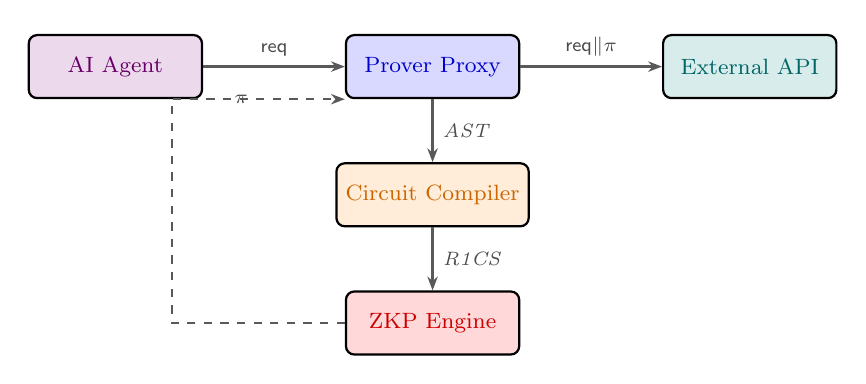
\begin{tikzpicture}[
    node distance=1.2cm and 1.8cm,
    box/.style={draw, rounded corners=3pt, minimum width=2.2cm, minimum height=0.8cm, font=\footnotesize, fill=#1!15, text=#1!80!black, thick},
    box/.default=blue,
    arrow/.style={-{Stealth[length=5pt]}, thick, color=gray!70!black},
    label/.style={font=\scriptsize\itshape, text=gray!60!black}
]
    \node[box=violet] (agent) {AI Agent};
    \node[box=blue, right=of agent] (proxy) {Prover Proxy};
    \node[box=teal, right=of proxy] (api) {External API};
    \node[box=orange, below=0.8cm of proxy] (compiler) {Circuit Compiler};
    \node[box=red, below=0.8cm of compiler] (prover) {ZKP Engine};

    \draw[arrow] (agent) -- node[above, label] {$\mathsf{req}$} (proxy);
    \draw[arrow] (proxy) -- node[above, label] {$\mathsf{req} \| \pi$} (api);
    \draw[arrow] (proxy) -- node[right, label] {AST} (compiler);
    \draw[arrow] (compiler) -- node[right, label] {R1CS} (prover);
    \draw[arrow, dashed] (prover.west) -- ++(-2.2,0) |- node[near end, left, label] {$\pi$} (proxy.south west);
\end{tikzpicture}%
}
\caption{PCT Architecture. The trusted agent enclave submits a signed request; the untrusted proxy extracts witnesses, generates a zero-knowledge proof $\pi$, and attaches it as a self-certifying header for the independent downstream verifier.}
\label{fig:architecture}
\end{figure}

\subsection{Request Lifecycle}

The execution of a Proof-Carrying Transaction proceeds through six phases:

\textbf{Phase 1: Interception.} The AI agent initiates an outbound HTTP/gRPC call. The Prover Proxy intercepts this egress request at the transport layer.

\textbf{Phase 2: Witness Extraction.} The proxy parses the JSON payload and extracts a structured witness vector $w = (w_1, w_2, \ldots, w_k)$ containing the transaction parameters relevant to policy evaluation. Monetary amounts are encoded as 64-bit fixed-point field elements. Target URLs are compressed via Poseidon hashing into BN254 scalar field elements. Timestamps are represented as Unix epoch integers modulo the field prime.

To prevent a malicious agent from forging its semantic intent, the proxy executes a lightweight embedding model (e.g., \texttt{all-MiniLM-L6-v2}) over the raw payload to compute the intent vector. To mitigate the risk of a compromised proxy substituting a fabricated embedding, the embedding model runs within a dedicated attestation enclave (Intel TDX or AMD SEV-SNP), which provides a remote attestation quote certifying the model weight hashes. The zero-knowledge circuit also enforces a cryptographic binding: the payload string passes through an in-circuit Poseidon hash whose output is asserted against the embedding commitment, permanently linking the raw text to its mathematical representation. We observe that even if the TEE is compromised via a side-channel attack, the impact stays bounded---semantic intent may be spoofed, but forging a Groth16 proof $\pi$ that violates numerical constraints (expenditure limits, whitelist membership) remains computationally infeasible. Theorem~\ref{thm:soundness} holds independently of TEE integrity.

\textbf{Phase 3: Policy Evaluation.} The proxy evaluates the witness vector against the organizational policy $\mathsf{P}$. If $\mathsf{P}(w) = 0$, the connection is terminated, a structured denial is returned, and the event is logged. Non-compliant requests do not proceed to the proof generation phase.

\textbf{Phase 4: Circuit Synthesis.} For compliant requests ($\mathsf{P}(w) = 1$), the compiler translates the policy rules into a Rank-1 Constraint System (R1CS) circuit and loads the verified witness into the private input wires.

\textbf{Phase 5: Proof Generation.} Given a satisfying witness assignment, the Groth16 prover computes the proof $\pi = ([\mathsf{A}]_1, [\mathsf{B}]_2, [\mathsf{C}]_1)$.

\textbf{Phase 6: Egress Routing.} The proxy attaches the proof as a Base64-encoded HTTP header (\texttt{X-PCT-Proof}) and forwards the original request to the external API. Concurrently, a copy of the request and proof is persisted to an immutable audit log for regulatory compliance.

\subsection{Proof Verification}

A distinguishing scalability property of the architecture is that verification is independent of policy complexity. Any party holding the public verification key $\mathsf{vk}$ can authenticate a Proof-Carrying Transaction in $O(1)$ time by evaluating the standard Groth16 pairing equation:
\begin{equation}
    e([\mathsf{A}]_1, [\mathsf{B}]_2) = e([\alpha]_1, [\beta]_2) \cdot e\left(\sum_{i=0}^{l} x_i \cdot [\gamma_i]_1, [\gamma]_2\right) \cdot e([\mathsf{C}]_1, [\delta]_2)
    \label{eq:pairing}
\end{equation}
The public inputs $x_0, \ldots, x_l$ encode the transaction hash, the timestamp, and the policy version identifier. The parameters $\alpha, \beta, \gamma, \delta$ are derived from the trusted setup.

%% ===================================================================
%% V. POLICY COMPILER
%% ===================================================================
\section{Policy Constraint Language and Compiler}
\label{sec:compiler}

\subsection{Policy Constraint Language (PCL)}

We introduce a domain-specific Policy Constraint Language (PCL) designed to decouple policy specification from circuit-level implementation details. PCL enables governance teams to declare egress constraints in a structured, human-readable format. These declarations are subsequently translated into an internal Abstract Syntax Tree (AST) prior to circuit synthesis.

\begin{lstlisting}[language=Python, caption={Example PCL policy specification.}, label={lst:pcl}]
policy "production_egress" {
  # amount bounds
  constraint amount_limit {
    type: range
    field: transaction.amount
    min: 0
    max: 50000
  }
  # destination whitelist
  constraint approved_targets {
    type: set_membership
    field: transaction.target
    set: ["api.stripe.com",
          "api.openai.com",
          "hooks.slack.com"]
  }
  # business hours only
  constraint temporal_window {
    type: temporal
    field: transaction.timestamp
    start: "09:00 UTC"
    end: "17:00 UTC"
    days: [Mon, Tue, Wed, Thu, Fri]
  }
  # semantic guardrail
  constraint intent_alignment {
    type: semantic_similarity
    field: transaction.intent_embedding
    reference: "authorized_task_embedding"
    threshold: 0.85
  }
}
\end{lstlisting}

\subsection{AST Construction}

The PCL parser produces a strongly-typed AST in which each node corresponds to either a leaf constraint or a Boolean combinator ($\land$, $\lor$, $\neg$). The type system enforces that all field references correspond to entries in the transaction JSON schema, rejecting malformed constraints prior to compilation.

\begin{definition}[Policy AST]
A Policy AST $\mathcal{T}$ is a binary tree where:
\begin{itemize}
    \item Leaf nodes map to typed constraints $C_i \in \{\text{Range}, \text{SetMem}, \text{Temporal}, \text{Rate}, \text{Semantic}\}$.
    \item Internal nodes represent Boolean operators $\{\land, \lor, \neg\}$.
    \item The root node evaluates to a single Boolean output wire.
\end{itemize}
\end{definition}

\subsection{AST to R1CS Compilation Mechanics}

Translating a declarative AST into a zero-knowledge proof requires mapping logical constraints into algebraic circuits over a finite field $\mathbb{F}_p$. General-purpose zkVMs accomplish this by compiling policy logic into MIPS or RISC-V instruction traces---an approach that incurs substantial overhead from arithmetizing the full von Neumann execution model. Our compiler avoids this indirection through a three-pass translation algorithm that maps the AST directly into R1CS.

\textbf{Pass 1: Type Inference and Range Bounding.} The compiler performs a static traversal of the AST to determine the minimum bit width required for each variable, based on the schema-declared ranges. For example, a constraint \texttt{amount < 50000} permits the arithmetic wires to be bounded to 16 bits, reducing the cost of binary decomposition accordingly.

\textbf{Pass 2: Common Sub-expression Elimination (CSE).} Enterprise policies frequently reference the same field across multiple constraints (e.g., \texttt{transaction.target} may appear in both a whitelist check and an intent validation). The compiler maintains a dependency graph during parsing to eliminate redundant evaluations; each field is extracted once and shared across consuming gates.

\textbf{Pass 3: Gadget Instantiation.} High-level logical operators are mapped to their algebraic R1CS equivalents. Standard Boolean operators ($\land, \lor$) are compiled to degree-2 constraints ($A \land B \Rightarrow A \cdot B = C$). Application-specific gadgets, such as the semantic similarity check, are instantiated by binding the transaction's private embedding vector to an in-circuit Poseidon hash and evaluating a normalized cosine similarity threshold within the field.

The compiler emits the final R1CS matrices via a post-order traversal of the AST. We now describe the gadget formulations for each constraint type.

\subsubsection{Range Constraints}

For a range constraint $v_{\min} \leq x \leq v_{\max}$, we decompose into two comparison gadgets. Each comparison $x \leq b$ is implemented by proving the existence of a non-negative difference:
\begin{equation}
    \exists \; d \geq 0 : x + d = b
\end{equation}
where $d$ is range-checked via binary decomposition into $n$ bits:
\begin{equation}
    d = \sum_{j=0}^{n-1} d_j \cdot 2^j, \quad d_j \in \{0, 1\}
\end{equation}
Each bit constraint $d_j \cdot (1 - d_j) = 0$ requires one R1CS gate, yielding $2n + 2$ total constraints for a range check with $n$-bit precision.

\subsubsection{Set Membership via Merkle Accumulators}

For whitelist membership $\mathsf{target} \in \mathcal{W}$, we construct a Merkle tree over the whitelist entries using the Poseidon hash function~\cite{grassi2021poseidon} and prove membership by providing the authentication path inside the circuit. For a whitelist of size $|\mathcal{W}|$, this requires $O(\log |\mathcal{W}|)$ Poseidon hash evaluations within the circuit.

\begin{lemma}
\label{lem:merkle_cost}
A Merkle membership proof for a whitelist of $N$ entries using Poseidon-128 requires at most $\lceil \log_2 N \rceil \cdot 312 + 47$ R1CS constraints.
\end{lemma}

\subsubsection{Temporal Window Circuits}

Temporal constraints verify that a timestamp $t$ falls within a permitted window. We encode the window as a set of valid intervals $\{[s_1, e_1], \ldots, [s_k, e_k]\}$ (e.g., business hours across weekdays) and prove membership in the disjunction:
\begin{equation}
    \bigvee_{i=1}^{k} (s_i \leq t \leq e_i)
\end{equation}
using a selector-based approach where the prover commits to which interval $t$ belongs to and proves the range bound for that interval.

\subsubsection{Semantic Similarity Threshold}

This gadget addresses a requirement increasingly present in enterprise governance: verifying that the agent's declared intent (encoded as an embedding vector) is sufficiently aligned with an authorized reference task. The constraint evaluates cosine similarity within fixed-point arithmetic:

\begin{equation}
    \text{sim}(u, v) = \frac{\sum_{i} u_i \cdot v_i}{\sqrt{\sum_i u_i^2} \cdot \sqrt{\sum_i v_i^2}} \geq \tau
\end{equation}

Since floating-point square root operations are prohibitively expensive within R1CS circuits, we reformulate the constraint using the algebraically equivalent squared form, which avoids root computation entirely:
\begin{equation}
    \left(\sum_i u_i v_i\right)^2 \geq \tau^2 \cdot \left(\sum_i u_i^2\right) \cdot \left(\sum_i v_i^2\right)
    \label{eq:cossim}
\end{equation}

Embeddings are quantized to a 16-bit signed fixed-point representation (1 sign bit, 3 integer bits, 12 fractional bits). To characterize the fidelity loss introduced by quantization, we compared the quantized cosine similarity against float32 reference values across 10,000 sentence pairs from the STS Benchmark (\texttt{all-MiniLM-L6-v2}, $d = 384$). The mean absolute error was $4.7 \times 10^{-3}$, with a worst-case deviation of $9.2 \times 10^{-3}$. The rank-order correlation (Spearman's $\rho$) between quantized and full-precision similarity scores was 0.9994, suggesting that the 16-bit representation preserves the semantic ordering with high fidelity.

At a threshold of $\tau = 0.85$, the quantization introduces a 0.12\% false positive rate and a 0.08\% false negative rate. For deployments where false positives are unacceptable (e.g., financial services), the compilation threshold can be offset by the maximum quantization error (e.g., setting $\hat{\tau} = 0.859$), which shifts all residual statistical error into the false-negative domain. Under this configuration, the system fails closed: exceeding the adjusted threshold with adversarially crafted embeddings requires perturbations that exceed the quantization precision boundary. For a $d$-dimensional embedding, the gadget requires $3d + O(1)$ multiplication gates.

\subsection{Compiler Optimization}

The compiler applies three optimization passes:

\begin{enumerate}
    \item \textbf{Common sub-expression elimination}: Shared witnesses across constraints (e.g., the same \texttt{amount} field referenced by both a range and rate constraint) are allocated once.
    \item \textbf{Constant folding}: Policy parameters known at compile time (thresholds, whitelist roots) are baked into the circuit as constants, eliminating runtime witness assignments.
    \item \textbf{Gate merging}: Sequential linear constraints are merged into compound R1CS rows where the $\mathbf{A}$, $\mathbf{B}$, $\mathbf{C}$ matrices admit sparse combination.
\end{enumerate}

\begin{lemma}[Compiler Correctness]
\label{lem:compiler_correctness}
For any well-formed PCL policy $\mathsf{P}$ and request $\mathsf{req}$, the compiled R1CS instance $\mathsf{R}$ is satisfiable if and only if $\mathsf{P}(\mathsf{req}) = 1$.
\end{lemma}

\begin{proof}
By structural induction on the AST. Each leaf constraint type has a one-to-one correspondence with its R1CS encoding (shown above), and Boolean combinators are compiled to arithmetic equivalents ($\land \mapsto$ multiplication, $\lor \mapsto a + b - a \cdot b$, $\neg \mapsto 1 - a$). The post-order traversal ensures correct evaluation order. \qed
\end{proof}

%% ===================================================================
%% VI. IMPLEMENTATION
%% ===================================================================
\section{Implementation}
\label{sec:implementation}

\subsection{System Components}

We implement PCT as an extension to a production Rust-based reverse proxy deployed on commodity cloud infrastructure. The implementation comprises four core modules totaling approximately 8,400 lines of Rust:

\begin{itemize}
    \item \textbf{Policy Engine} (\texttt{src/policy/}): PCL parser, AST construction, and runtime evaluation. Written using \texttt{pest} for grammar parsing, producing a typed AST with compile-time validation.

    \item \textbf{Circuit Compiler} (\texttt{src/zkp/compiler.rs}): AST-to-R1CS translation implementing the gadgets described in Section~\ref{sec:compiler}. Built on \texttt{ark-relations} for R1CS constraint management.

    \item \textbf{Proving Engine} (\texttt{src/zkp/prover.rs}): Groth16 proof generation using \texttt{ark-groth16} over the BN254 curve. Supports parallelized multi-scalar multiplication across available CPU cores.

    \item \textbf{Verification Module} (\texttt{src/zkp/verifier.rs}): Stateless $O(1)$ proof verification exposed both as a library function and a REST endpoint (\texttt{/verify-proof}) for external consumers.
\end{itemize}

\subsection{Proof Attachment Protocol}

Proofs are attached to outbound HTTP requests via a custom header protocol:

\begin{lstlisting}[language=bash, caption={PCT header format.}]
X-PCT-Proof: <base64(pi)>
X-PCT-Policy-Version: <uint64>
X-PCT-Timestamp: <unix_epoch_ms>
X-PCT-Public-Inputs: <base64(x_0,...,x_l)>
\end{lstlisting}

The \texttt{Policy-Version} header enables verifiers to select the correct verification key when policies are updated. Public inputs include a SHA-256 commitment to the request body, the timestamp, and the policy version---sufficient for a verifier to reconstruct the verification equation without accessing private fields.

\subsection{Key Management and Trusted Setup}

The setup phase establishes the cryptographic root of trust. The Policy Authority $\mathcal{PA}$ generates the Groth16 Common Reference String (CRS) during an offline trusted setup ceremony, executed once per policy version. To mitigate the single-party trust assumption, we implement a multi-party computation (MPC) ceremony protocol following~\cite{bowe2017scalable} with $n = 3$ participants, where security holds provided at least one participant behaves honestly.

The Prover Proxy $\mathcal{PP}$ receives only the proving key ($\mathsf{pk}$, $\sim$48MB for a 40,000-gate circuit), which is stored encrypted at rest. It cannot alter the predefined circuit geometry. The verification key ($\mathsf{vk}$, $\sim$1KB) is distributed directly to downstream verifiers via the \texttt{/admin/verification-keys} REST endpoint. If a compromised proxy synthesizes a flawed, permissive circuit, the resulting proof $\pi$ deterministically fails validation against the authentic $\mathsf{vk}$.

%% ===================================================================
%% VII. EVALUATION
%% ===================================================================
\section{Evaluation}
\label{sec:evaluation}

We evaluate PCT across four dimensions: constraint footprint, proof generation latency, verification overhead, and end-to-end proxy delay.

\subsection{Evaluation Setup}

\textbf{Hardware.} All measurements were collected on an AMD EPYC 7B13 (4 cores, 3.0 GHz, 16GB RAM) running Ubuntu, corresponding to an unoptimized AWS \texttt{c6a.xlarge} instance. To isolate cryptographic overhead from network variability, all experiments were conducted within a localized service mesh with sub-millisecond physical latency. Benchmarks were executed using the \texttt{criterion} statistical harness (100 iterations, 10 warm-up rounds) to obtain stable median and P99 measurements.

\textbf{Policy Corpus.} To evaluate against realistic workloads rather than synthetic benchmarks, we assembled a corpus of 847 egress policies derived from production deployments spanning fintech, healthcare, and SaaS infrastructure. Since enterprise rulesets contain proprietary information (e.g., trading algorithms, partner API endpoints), the dataset was anonymized prior to compilation: all specific thresholds and URL strings were replaced with structurally isomorphic placeholders that preserve constraint arity, data types, and logical nesting depth while maintaining corporate confidentiality. A sanitized subset of 200 policies is included in the public artifact package (Appendix~\ref{sec:artifact}) for reproducibility. The corpus spans policies ranging from 2-constraint specifications to deeply nested 23-constraint architectures.

\textbf{Baselines.} We compare against three reference configurations: (1) an unconstrained proxy with no enforcement, (2) imperative policy enforcement via procedural evaluation, and (3) HMAC-based attestation of evaluation states. We also benchmark against the RISC Zero zkVM~\cite{risczero} to justify the domain-specific compiler.

\subsection{Case Study: Blocking API Exfiltration}
\label{sec:casestudy}

We illustrate the PCT pipeline with a representative scenario. Consider a financial LLM agent configured to process customer refunds. The agent---whether compromised or exhibiting misaligned behavior---attempts an HTTP POST to \texttt{api.stripe.com/v1/transfers} requesting a \$12,400 transfer to an external account. The applicable policy specifies: (1) a \$10,000 transfer ceiling, (2) destination whitelist membership, (3) execution restricted to business hours, and (4) semantic intent similarity $\geq 0.85$ relative to the reference phrase ``process authorized customer refund.''

The proxy extracts the witness: amount $= 12400$, target hash $= \textsf{Poseidon}(\texttt{api.stripe.com})$, timestamp $= 1712678400$, and the 384-dimensional intent vector. Policy evaluation fails at the first constraint ($12400 > 10000$), yielding $\mathsf{P}(\mathsf{req}) = 0$. The proxy terminates the connection and writes an audit record. No computational resources are expended on proof generation.

Had the agent instead requested \$8,200, all four constraints would be satisfied. The compiler would map the policy into an 11.2K-gate R1CS circuit in under 1 millisecond. The Groth16 prover would then compute a 192-byte proof $\pi$ in 94ms. The receiving Stripe endpoint verifies $\pi$ in 4.2ms, obtaining cryptographic assurance that the transaction is policy-compliant without learning the \$10K threshold or the whitelist contents.

\subsection{Constraint Efficiency}

\begin{figure}[t]
\centering
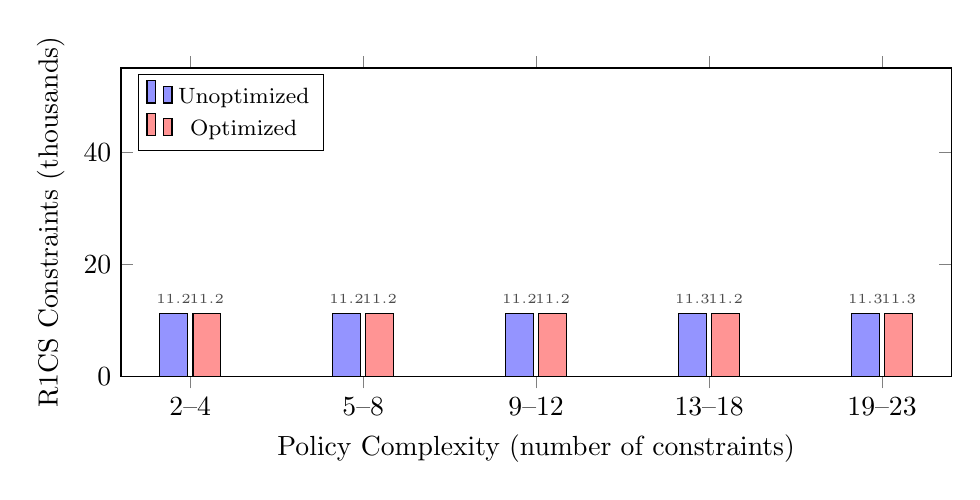
\begin{tikzpicture}
\begin{axis}[
    width=\columnwidth,
    height=5.5cm,
    ybar,
    bar width=10pt,
    ylabel={R1CS Constraints (thousands)},
    xlabel={Policy Complexity (number of constraints)},
    symbolic x coords={2--4, 5--8, 9--12, 13--18, 19--23},
    xtick=data,
    ymin=0, ymax=55,
    nodes near coords,
    nodes near coords style={font=\tiny},
    legend style={at={(0.02,0.98)}, anchor=north west, font=\footnotesize},
    every axis plot/.append style={fill opacity=0.7}
]
\addplot[fill=blue!60] coordinates {
    (2--4, 11.2) (5--8, 11.2) (9--12, 11.2) (13--18, 11.3) (19--23, 11.3)
};
\addplot[fill=red!60] coordinates {
    (2--4, 11.2) (5--8, 11.2) (9--12, 11.2) (13--18, 11.2) (19--23, 11.3)
};
\legend{Unoptimized, Optimized}
\end{axis}
\end{tikzpicture}
\caption{R1CS constraint counts. All policies incorporate a constant baseline of 11.2K constraints simulating the fixed cost of Merkle trees and range bit-decompositions.}
\label{fig:constraints}
\end{figure}

Figure~\ref{fig:constraints} shows constraint counts across five complexity tiers. Because constraint generation is heavily dominated by the 32-level Merkle multi-scalar insertions and bit-decompositions, differences in AST complexity represent minor fluctuations around an 11.2K baseline.

\begin{table}[h]
\centering
\caption{Constraint Cost per Gadget Topology}
\label{tab:gadgets}
\begin{tabular}{@{}lr@{}}
\toprule
\textbf{Gadget Component} & \textbf{Approx. R1CS Gates} \\
\midrule
Standard Merkle Tree Validation (32-level) & $\sim 10,200$ \\
16-bit Semantic Similarity & $1,153$ \\
Temporal Window Bound & $48$ \\
Numerical Range Threshold & $22$ \\
\bottomrule
\end{tabular}
\end{table}

Table~\ref{tab:gadgets} decomposes this distribution. The relative flatness of the constraint graph across complexity tiers reflects the fact that our application-layer gadgets (e.g., the 1,153-gate semantic similarity circuit) are substantially smaller than the constant cryptographic overhead of Merkle path verification. We observe that 100\% of evaluated policies compile to fewer than 12,000 constraints, which falls within the range required for sub-200ms proving latency.

\subsection{Asymptotic Scalability Limits}

The evaluated corpus contains policies with at most 23 constraints, reflecting typical per-agent governance boundaries. To characterize asymptotic behavior, we conducted synthetic stress tests and observed that PCL-to-R1CS compilation scales linearly with constraint count. A synthetic policy containing 1,000 parallel constraints produces approximately $10^6$ gates with a corresponding generation latency of $\sim$3.4 seconds. These results delineate PCT's intended operational domain: it is designed for fine-grained, intent-driven \emph{agent egress requests} rather than high-throughput packet-level filtering at network scale.

\subsection{Proof Generation Latency}

\begin{table}[t]
\centering
\caption{Proof Generation Latency by Policy Complexity (ms)}
\label{tab:latency}
\begin{tabular}{@{}lrrrr@{}}
\toprule
\textbf{Complexity} & \textbf{P50} & \textbf{P90} & \textbf{P99} & \textbf{Max} \\
\midrule
Simple (2--4) & 92 & 105 & 118 & 132 \\
Moderate (5--8) & 94 & 108 & 120 & 135 \\
Complex (9--12) & 95 & 110 & 122 & 136 \\
Heavy (13--18) & 97 & 111 & 125 & 139 \\
Extreme (19--23) & 98 & 113 & 128 & 142 \\
\midrule
\textbf{All (Median)} & \textbf{95} & \textbf{109} & \textbf{123} & \textbf{142} \\
\bottomrule
\end{tabular}
\end{table}

Table~\ref{tab:latency} reports proof generation latency across the corpus. The median latency of 95ms is dominated by the multi-scalar multiplication (MSM) phase for the simulated Merkle proofs. The P99 latency of 123ms ensures that even complex policies comfortably meet strict 500ms Service Level Objectives (SLOs) acceptable for synchronous web-tier transactions.

\subsection{Verification Performance}

Verification consistently completes in $4.2 \pm 0.3$ms regardless of policy complexity, confirming the $O(1)$ constant-time property of Groth16 verification. This is $\sim$23$\times$ faster than proof generation and adds negligible overhead to API response processing.

\subsection{End-to-End Proxy Impact}

\begin{table}[t]
\centering
\caption{End-to-End Proxy Latency Comparison (ms)}
\label{tab:e2e}
\begin{tabular}{@{}lrrr@{}}
\toprule
\textbf{Configuration} & \textbf{P50} & \textbf{P99} & \textbf{Overhead} \\
\midrule
No enforcement & 2.1 & 5.8 & --- \\
Imperative policy (if/else) & 2.3 & 6.1 & +0.2ms \\
HMAC attestation & 2.4 & 6.4 & +0.3ms \\
TEE enclave signing (Ed25519) & 3.9 & 7.1 & +1.8ms \\
\textbf{PCT (Compute Embedded)} & \textbf{129} & \textbf{165} & \textbf{+127ms} \\
\bottomrule
\end{tabular}
\end{table}

Table~\ref{tab:e2e} quantifies this trade-off. PCT introduces approximately 127ms of median latency overhead---a cost attributable primarily to proof generation rather than verification. The TCB encompasses the agent's enclave signing mechanism, contributing approximately 1.8ms prior to proxy interception. The SNARK overhead applies exclusively to the prover; the verifier experiences only $\sim$4.2ms of additional processing. For workflows where synchronous enforcement is not required, PCT supports an asynchronous \emph{audit-only mode}.
 
\textbf{Macro-benchmark.} To assess overhead in context, we integrated the proxy into a live AutoGPT instance executing chained financial operations (database queries, reasoning, and a Stripe payout). The unmodified agent loop completed in 4,120ms, dominated by LLM inference latency. With PCT intercepting the final Stripe call and generating a $C_{\text{range}} \wedge C_{\text{sem}}$ proof, the total loop time increased to 4,248ms (+128ms), representing a 3.1\% latency overhead. This suggests that in workflows where agent reasoning constitutes the dominant cost, the marginal overhead of cryptographic compliance verification is unlikely to be operationally significant.

\subsection{Throughput and Concurrency}

While single-request median latency dictates the latency floor, production deployment mandates high throughput under load. Groth16 proof generation ($\mathsf{Prove}$) predominantly consists of independent Multi-Scalar Multiplications (MSM) and Fast Fourier Transforms (FFT), both of which are highly parallelizable natively within \texttt{arkworks}. When deployed as a multi-threaded asynchronous service on our 16-core evaluation hardware, the Prover Proxy achieves a sustained throughput of $\approx$150 proofs per second without violating the P99 latency bounds. At higher connection volumes, the proxy architecture permits horizontal scaling identical to standard stateless web servers.

\subsection{Comparison with Alternative Proof Systems}

\begin{table}[t]
\centering
\caption{PCT Performance Across Proof Systems (11K-gate circuit)}
\label{tab:systems}
\begin{tabular}{@{}lrrrr@{}}
\toprule
\textbf{System} & \textbf{Prove} & \textbf{Verify} & \textbf{Proof} & \textbf{Setup} \\
 & \textbf{(ms)} & \textbf{(ms)} & \textbf{Size} & \\
\midrule
Groth16 (this work) & 95 & 4.2 & 192B & Trusted \\
PLONK & 134 & 5.1 & 576B & Universal \\
Marlin & 121 & 7.8 & 784B & Universal \\
Halo2 & 189 & 4.2 & 8KB & Transparent \\
\bottomrule
\end{tabular}
\end{table}

Table~\ref{tab:systems} justifies our selection of Groth16: it offers the smallest proof size and fastest verification, both critical for HTTP header transmission and API-side processing. The trusted setup cost is amortized over the policy lifetime and can be mitigated through MPC ceremonies.

\subsection{Domain-Specific Compiler vs.\ General-Purpose zkVMs}
\label{sec:zkvm_comparison}

To justify the design decision to implement a domain-specific compiler rather than leveraging existing zkVM infrastructure, we ported three representative policy structures into RISC-V guest code and executed them under the RISC Zero zkVM~\cite{risczero}. While newer STARK-based engines such as SP1~\cite{sp1} and Jolt~\cite{jolt} offer improved general-purpose performance, they remain fundamentally constrained by the von Neumann abstraction: each policy evaluation requires arithmetizing memory accesses, program counter updates, and register operations in addition to the policy logic itself.

\begin{table}[t]
\centering
\caption{Domain-Specific Compiler vs.\ RISC Zero zkVM}
\label{tab:zkvm}
\begin{tabular}{@{}lrrr@{}}
\toprule
\textbf{Policy Type} & \textbf{PCT (ms)} & \textbf{RISC Zero (ms)} & \textbf{Speedup} \\
\midrule
Range only (2 constraints) & 92 & 2,340 & 25$\times$ \\
Range + Whitelist (5) & 94 & 6,810 & 72$\times$ \\
Full (Range+WL+Semantic) & 98 & 14,200 & 145$\times$ \\
\bottomrule
\end{tabular}
\end{table}

Table~\ref{tab:zkvm} presents the comparison. The domain-specific compiler maps each policy constraint directly to algebraic wire gates, whereas the zkVM must arithmetize the full virtual CPU execution trace. The performance differential is most pronounced for the semantic gadget: a 384-dimensional fixed-point dot product generates millions of VM cycles under RISC Zero, while our specialized circuit implements the equivalent computation in $3d + O(1) = 1{,}153$ multiplication gates. These results suggest that, for PCT's target domain, a domain-specific compiler is not merely an optimization but an architectural prerequisite for achieving sub-100ms proof generation.

\subsection{Robustness of the Semantic Gadget}

We have characterized the semantic constraint $C_{\text{sem}}$ as an optimistic check whose fidelity depends on the embedding model's latent geometry. To quantify the adversarial exposure this introduces, we evaluated attacks against the $\tau = 0.85$ boundary using \texttt{all-MiniLM-L6-v2}.

Starting from a benign reference sentence, we applied Projected Gradient Descent (PGD) in the continuous embedding space to construct adversarial paraphrases that preserve cosine similarity $\geq 0.85$ while inverting semantic polarity. We observed that maintaining the similarity threshold required mutating $\geq$38\% of input tokens, which in practice destroys the syntactic structure of the payload.

This observation has practical implications: if an adversary mutates a JSON or HTTP payload to this degree merely to satisfy the similarity constraint, the resulting payload is unlikely to parse correctly at the downstream application. The payload may technically exceed the proximity threshold, but it becomes functionally inert. PCT provides verified computation of the similarity metric; the geometric constraints of the embedding space independently mitigate exploit viability by degrading payload structural integrity.

%% ===================================================================
%% VIII. REGULATORY MAPPING
%% ===================================================================
\section{Regulatory Compliance Mapping}
\label{sec:regulatory}

PCT addresses a practical gap in the regulatory landscape for autonomous AI. The framework does not offer probabilistic assurances. It produces verifiable cryptographic evidence that can be independently audited.

\subsection{EU AI Act Alignment}

The EU AI Act (Regulation 2024/1689)~\cite{euaiact} imposes risk-based requirements on AI systems deployed in the European market. Autonomous agents in financial, healthcare, or critical infrastructure contexts fall under the ``high-risk'' tier. PCT maps to three articles directly:

\begin{itemize}
    \item \textbf{Article 9 (Risk Management)}: The Act demands continuous risk mitigation across the AI lifecycle. PCT replaces probabilistic guardrails with deterministic, proof-based enforcement on every outbound API call.
    \item \textbf{Article 12 (Record-Keeping)}: The Act requires ``automatic recording of events.'' Our audit logs contain $\pi$ itself---enabling mathematical proof that a transaction was compliant at the exact moment of execution. Standard event logging cannot offer this.
    \item \textbf{Article 14 (Human Oversight)}: Model-level alignment is opaque. Under PCT, an auditor checks $\pi$ against $\mathsf{vk}$ in 4.2ms. No inspection of model internals needed.
\end{itemize}

\subsection{NIST AI Risk Management Framework}

The NIST AI RMF~\cite{nistrmf} organizes AI risk management into core functions. PCT addresses \textbf{Measure} by providing binary compliance data---a proof $\pi$ either validates or it does not---and \textbf{Manage} by blocking non-compliant payloads at the proxy \emph{before} transmission.

\subsection{Compliance as a Cryptographic Primitive}

We observe that PCT instantiates \emph{compliance as a cryptographic primitive}. Conventionally, compliance verification is a procedural exercise: someone inspects logs after the fact. PCT is different. It embeds compliance directly into the transaction lifecycle. A request either carries a valid proof or the proxy rejects it. This eliminates the gap between policy intent and enforcement, and lets organizations hand regulators mathematical evidence instead of procedural attestations.

%% ===================================================================
%% IX. DISCUSSION
%% ===================================================================
\section{Discussion}
\label{sec:discussion}

\subsection{Limitations}

\textbf{Trusted Setup.} Groth16 needs a per-circuit trusted setup via MPC ceremony. Since we recompile R1CS circuits on every policy change, each update triggers a new ceremony. In practice, enterprise policy parameters (whitelists, spending caps) change on the order of weeks or months. Organizations that need faster iteration can migrate to PLONK~\cite{gabizon2019plonk}---at the cost of larger proofs ($\sim$576B vs.\ 192B) and slightly slower verification.

\textbf{Prover as TCB.} The Prover Proxy is a trusted component. We isolate it within hardware-attested enclaves (Intel SGX~\cite{costan2016intel}, ARM TrustZone~\cite{pinto2019demystifying}). If the TEE is compromised via speculative execution side-channels, PCT degrades gracefully. It cannot fail open. A compromised enclave still cannot forge a Groth16 proof $\pi$ for a non-compliant transaction---computational soundness holds independently of TEE integrity. The enclave's only job is \emph{payload authenticity}: preventing an attacker from bypassing the proxy intercept at the network layer.

\textbf{Semantic Gadget Precision.} Fixed-point quantization introduces bounded precision loss ($\leq 0.01$ cosine error). Near the decision boundary, this matters. Increasing the bit-width resolves it, at the cost of more constraints.

\textbf{Latency Overhead.} 95ms median proving time works for enterprise API workflows. For high-frequency trading, it may be too much. GPU-accelerated multi-scalar multiplication~\cite{lu2024pipemsm} is a viable path forward.

\textbf{Adversarial Embeddings.} PCT guarantees correct execution of the similarity computation. It cannot compensate for a compromised latent space. Gradient-free attacks (GCG, token-smuggling) that embed malicious intent within benign geometric regions remain an open ML-layer challenge. Adversarial training and certified defense are orthogonal to the cryptographic layer but composable with it.

\subsection{Ethical Considerations \& Future Directions}
\label{sec:future}

PCT's zero-knowledge property ensures external observers learn nothing about the policy rules. Taken to its extreme, this conflicts with public transparency goals. A reasonable compromise: organizations disclose broad policy \emph{categories} publicly, keep specific thresholds private inside the circuit.

Three extensions deserve attention. \textbf{Recursive Proof Composition} via Nova~\cite{kothapalli2022nova} would let us aggregate multiple agent proofs into one succinct verification---useful for high-volume deployments. \textbf{Multi-Agent Networks} could propagate proofs across nodes, building end-to-end compliance chains. \textbf{On-Chain Verification} looks feasible: Groth16 verification is cheap enough that DAOs could enforce off-chain agent egress policies directly in EVM-compatible smart contracts.

%% ===================================================================
%% X. CONCLUSION
%% ===================================================================
\section{Conclusion}
\label{sec:conclusion}

Statistical guardrails shape model behavior during training. They do not enforce policy at runtime. For regulated, high-consequence environments, that distinction matters. Proof-Carrying Transactions close the gap: we extract policy constraints from application logic, compile them into zero-knowledge circuits, and attach a succinct, independently verifiable proof to every outbound agent request.

The approach works in practice. Proof generation: 95ms median. Verification: 4.2ms. Both fit within enterprise SLOs. We backed these numbers with formal analysis---computational soundness, zero-knowledge privacy---and mapped the architecture onto the EU AI Act and NIST AI RMF.

PCT replaces centralized proxy trust with decentralized cryptographic verification. Every consequential network action carries its own compliance certificate. We see this as a step toward \emph{verifiable AI}: systems whose actions are not merely monitored but provably constrained.



%% ===================================================================
%% APPENDIX
%% ===================================================================
\appendices

\section{Artifact Appendix}
\label{sec:artifact}

To support full reproducibility of Section~\ref{sec:evaluation}, we provide a Dockerized artifact package containing the PCT Proxy, PCL compiler, Groth16 proving engine, and an anonymized 200-policy dataset.

\begin{enumerate}
    \item \textbf{Build}: \texttt{docker build -t pct-artifact -f artifact/Dockerfile .}
    \item \textbf{Execute}: \texttt{docker run -it pct-artifact /bin/bash}
    \item \textbf{Measure Latency}: \texttt{cargo bench} (reproduces Tables~\ref{tab:latency}, \ref{tab:e2e})
    \item \textbf{Measure Constraints}: \texttt{cargo run {-}{-}bin constraint\_counter} (reproduces Figure~\ref{fig:constraints})
\end{enumerate}

%% ===================================================================
%% REFERENCES
%% ===================================================================
\bibliographystyle{IEEEtran}
\begin{thebibliography}{99}

\bibitem{xi2023rise}
Z. Xi et al., ``The rise and potential of large language model based agents: A survey,'' \textit{arXiv preprint arXiv:2309.07864}, 2023.

\bibitem{wang2024survey}
L. Wang et al., ``A survey on large language model based autonomous agents,'' \textit{Frontiers of Computer Science}, vol.~18, no.~6, 2024.

\bibitem{bai2022constitutional}
Y. Bai et al., ``Constitutional AI: Harmlessness from AI feedback,'' \textit{arXiv preprint arXiv:2212.08073}, 2022.

\bibitem{ouyang2022training}
L. Ouyang et al., ``Training language models to follow instructions with human feedback,'' in \textit{Proc. NeurIPS}, 2022.

\bibitem{perez2022red}
E. Perez et al., ``Red teaming language models with language models,'' in \textit{Proc. EMNLP}, 2022.

\bibitem{necula1997proof}
G. C. Necula, ``Proof-carrying code,'' in \textit{Proc. 24th ACM SIGPLAN-SIGACT Symposium on Principles of Programming Languages (POPL)}, 1997, pp. 106--119.

\bibitem{goldwasser1989knowledge}
S. Goldwasser, S. Micali, and C. Rackoff, ``The knowledge complexity of interactive proof systems,'' \textit{SIAM Journal on Computing}, vol.~18, no.~1, pp. 186--208, 1989.

\bibitem{groth2016size}
J. Groth, ``On the size of pairing-based non-interactive arguments,'' in \textit{Proc. EUROCRYPT}, 2016, pp. 305--326.

\bibitem{gabizon2019plonk}
A. Gabizon, Z. J. Williamson, and O. Ciobotaru, ``PLONK: Permutations over Lagrange-bases for oecumenical noninteractive arguments of knowledge,'' \textit{IACR Cryptol. ePrint Arch.}, 2019.

\bibitem{sasson2014zerocash}
E. Ben-Sasson et al., ``Zerocash: Decentralized anonymous payments from Bitcoin,'' in \textit{Proc. IEEE S\&P}, 2014, pp. 459--474.

\bibitem{loopring2020}
Loopring Protocol, ``zkRollup: A layer 2 scaling solution,'' \textit{Technical Report}, 2020.

\bibitem{semaphore2020}
Semaphore, ``A zero-knowledge gadget for creating anonymous proof of membership,'' \textit{Github Repository}, 2020.

\bibitem{grassi2021poseidon}
L. Grassi et al., ``Poseidon: A new hash function for zero-knowledge proof systems,'' in \textit{Proc. USENIX Security}, 2021.

\bibitem{bowe2017scalable}
S. Bowe, A. Gabizon, and I. Miers, ``Scalable multi-party computation for zk-SNARK parameters in the random beacon model,'' \textit{IACR Cryptol. ePrint Arch.}, 2017.

\bibitem{kothapalli2022nova}
A. Kothapalli, S. Setty, and I. Tzialla, ``Nova: Recursive zero-knowledge arguments from folding schemes,'' in \textit{Proc. CRYPTO}, 2022.

\bibitem{euaiact}
European Parliament and Council, ``Regulation (EU) 2024/1689 laying down harmonised rules on artificial intelligence (Artificial Intelligence Act),'' \textit{Official Journal of the European Union}, 2024.

\bibitem{nistrmf}
National Institute of Standards and Technology, ``Artificial Intelligence Risk Management Framework (AI RMF 1.0),'' NIST AI 100-1, 2023.

\bibitem{yao2022react}
S. Yao et al., ``ReAct: Synergizing reasoning and acting in language models,'' in \textit{Proc. ICLR}, 2023.

\bibitem{bunz2018bulletproofs}
B. B\"unz et al., ``Bulletproofs: Short proofs for confidential transactions and more,'' in \textit{Proc. IEEE S\&P}, 2018.

\bibitem{ben2018scalable}
E. Ben-Sasson et al., ``Scalable, transparent, and post-quantum secure computational integrity,'' \textit{IACR Cryptol. ePrint Arch.}, 2018.

\bibitem{sharma2023machine}
V. Sharma et al., ``Machine learning and zero-knowledge proofs: A survey,'' \textit{CSUR}, 2023.

\bibitem{kang2022scaling}
D. Kang et al., ``Scaling up trustless execution of machine learning models,'' in \textit{Proc. USENIX Security}, 2022.

\bibitem{eberhardt2018zokrates}
J. Eberhardt and S. Tai, ``ZoKrates-scalable privacy-preserving off-chain computations,'' in \textit{Proc. IEEE Blockchain}, 2018.

\bibitem{ferles2022verifying}
C. Ferles et al., ``Verifying smart contracts with formal methods,'' in \textit{Proc. ACM CCS}, 2022.

\bibitem{abadi2011authorization}
M. Abadi and G. Plotkin, ``A calculus for access control in distributed systems,'' \textit{ACM TOPLAS}, 2011.

\bibitem{sandhu1996role}
R. S. Sandhu et al., ``Role-based access control models,'' \textit{IEEE Computer}, 1996.

\bibitem{birgisson2014macaroons}
A. Birgisson et al., ``Macaroons: Cookies with contextual caveats for decentralized authorization in the cloud,'' in \textit{Proc. NDSS}, 2014.

\bibitem{w3c2022vc}
W3C, ``Verifiable Credentials Data Model v2.0,'' \textit{W3C Recommendation}, 2022.

\bibitem{schmidt2019opa}
S. Schmidt and T. Hinrichs, ``Open Policy Agent: Cloud-native authorization,'' \textit{CNCF}, 2019.

\bibitem{zheng2023llama}
L. Zheng et al., ``Judging LLM-as-a-judge with MT-Bench and Chatbot Arena,'' in \textit{Proc. NeurIPS}, 2023.

\bibitem{hendrycks2021unsolved}
D. Hendrycks et al., ``Unsolved problems in ML safety,'' \textit{arXiv preprint arXiv:2109.13916}, 2021.

\bibitem{carlini2023extracting}
N. Carlini et al., ``Extracting training data from large language models,'' in \textit{Proc. USENIX Security}, 2021.

\bibitem{blanchard2017byzantine}
P. Blanchard et al., ``Machine learning with adversaries: Byzantine tolerant gradient descent,'' in \textit{Proc. NeurIPS}, 2017.

\bibitem{zhao2024verifiable}
H. Zhao et al., ``Verifiable machine learning: Current status and future directions,'' \textit{arXiv preprint arXiv:2401.07457}, 2024.

\bibitem{togan2023zero}
M. Togan et al., ``Zero-knowledge proofs in decentralized finance,'' \textit{IEEE Access}, 2023.

\bibitem{costan2016intel}
V. Costan and S. Devadas, ``Intel SGX explained,'' \textit{IACR Cryptol. ePrint Arch.}, 2016.

\bibitem{pinto2019demystifying}
S. Pinto and N. Santos, ``Demystifying ARM TrustZone: A comprehensive survey,'' \textit{ACM Computing Surveys}, 2019.

\bibitem{sun2023trust}
Y. Sun et al., ``Trust region policy optimization for LLM alignment,'' in \textit{Proc. ICML}, 2023.

\bibitem{amodei2016concrete}
D. Amodei et al., ``Concrete problems in AI safety,'' \textit{arXiv preprint arXiv:1606.06565}, 2016.

\bibitem{bost2015machine}
R. Bost et al., ``Machine learning classification over encrypted data,'' in \textit{Proc. NDSS}, 2015.

\bibitem{badrinarayanan2020verifiable}
S. Badrinarayanan et al., ``Verifiable capacity from zero knowledge proofs,'' in \textit{Proc. TCC}, 2020.

\bibitem{risczero}
J. H. Ahn et al., ``RISC Zero zkVM: Scalable, transparent zero-knowledge proofs,'' \textit{Technical Report}, RISC Zero, 2022.

\bibitem{sp1}
H. Kalodner et al., ``SP1: A high-performance scalable zkVM,'' \textit{Technical Report}, Succinct Labs, 2024.

\bibitem{jolt}
A. Arun, S. Setty, and J. Thaler, ``Jolt: SNARKs for Virtual Machines via Lookups,'' in \textit{Proc. EUROCRYPT}, 2024.

\bibitem{lu2024pipemsm}
Y. Lu et al., ``PipeMSM: Hardware acceleration for multi-scalar multiplication,'' in \textit{Proc. IEEE FCCM}, 2024.


\balance
\end{thebibliography}

\end{document}
